\documentclass[conference]{IEEEtran}
\usepackage{times}
\usepackage[numbers]{natbib}
\usepackage{multicol}
\usepackage[bookmarks=true]{hyperref}
\usepackage{graphicx}
\usepackage{amsmath}
\usepackage{algorithm}
\usepackage{algpseudocode}
\usepackage{booktabs}

\pdfinfo{
   /Author (Anonymous)
   /Title  (Autonomous Frontier-Based Exploration in ROS2)
   /CreationDate (D:20251022000000)
   /Subject (Robotics)
   /Keywords (Autonomous Exploration;ROS2;Frontier-Based Navigation;SLAM)
}

\begin{document}

\title{Autonomous Frontier-Based Exploration\\ in ROS2: System Integration and Performance Analysis}

\author{Author Names Omitted for Anonymous Review. Paper-ID [TBD]}

\maketitle

\begin{abstract}
This milestone report presents our progress in implementing and evaluating an autonomous exploration system for mobile robots using ROS2. We adapted the m-explore package, a frontier-based exploration algorithm, and successfully deployed it in simulation with the TurtleBot3 platform. Our preliminary results demonstrate automated exploration achieving 74.3\% environment coverage in 185 seconds, outperforming manual teleoperation by 2.2$\times$ in exploration efficiency. We integrated SLAM, navigation, and exploration components into a cohesive system and developed metrics collection tools to quantify exploration performance. Key challenges identified include exploration speed optimization and parameter tuning for different environments.
\end{abstract}

\IEEEpeerreviewmaketitle

\section{Introduction}

Autonomous exploration enables robots to systematically discover and map unknown environments without human intervention, a fundamental capability for applications ranging from search and rescue to planetary exploration. Our project focuses on implementing and analyzing frontier-based exploration in ROS2, where frontiers represent the boundaries between explored free space and unexplored regions.

Since our initial proposal, we have successfully integrated the exploration system, conducted preliminary experiments, and identified key performance bottlenecks. This milestone report details our technical implementation, presents quantitative results from simulation experiments, and outlines our path toward optimizing exploration efficiency.

\section{Problem Refinement \& Objectives}

\subsection{Evolved Problem Statement}

Our initial proposal aimed to implement autonomous exploration in ROS2. Through hands-on development, we have refined this to focus on three interconnected challenges:

\textbf{System Integration:} Coordinating SLAM (Simultaneous Localization and Mapping), path planning (Nav2), and frontier detection into a robust exploration pipeline that handles dynamic environments and recovers from navigation failures.

\textbf{Performance Optimization:} Addressing exploration speed bottlenecks observed in our initial trials, where the robot explores "suuuper slowly" compared to expectations—potentially due to computational constraints, parameter misconfiguration, or algorithmic inefficiencies.

\textbf{Quantitative Evaluation:} Developing metrics and benchmarks to objectively assess exploration performance across different environments and parameter configurations.

\subsection{Refined Objectives}

Based on early implementation experience, our specific objectives for this project are:

\begin{enumerate}
\item \textbf{Deploy functional exploration system:} Integrate m-explore-ros2 with Nav2 and SLAM backends (slam\_toolbox/cartographer) in simulation (\textit{Completed}).

\item \textbf{Implement performance monitoring:} Create real-time metrics collection for coverage, exploration rate, and efficiency analysis (\textit{Completed}).

\item \textbf{Conduct comparative analysis:} Quantify autonomous vs. manual exploration to establish baseline performance (\textit{In Progress}).

\item \textbf{Optimize exploration parameters:} Systematically tune frontier selection criteria, planning frequency, and navigation parameters to improve exploration speed (\textit{Milestone 2}).

\item \textbf{Evaluate multi-environment generalization:} Test performance across varied environment complexities and sizes (\textit{Milestone 2 \& Final}).
\end{enumerate}

\section{Technical Implementation}

\subsection{System Architecture}

Our exploration system builds upon the m-explore-ros2 package, a ROS2 port of the frontier-based exploration algorithm originally developed for ROS1~\cite{horner2016exploration}. The architecture comprises four main components:

\textbf{SLAM Backend:} We use ROS2 Cartographer for real-time mapping and localization. The SLAM system subscribes to laser scan data and odometry, publishing occupancy grid maps that distinguish free space (-1: unknown, 0: free, 100: occupied) and robot pose estimates.

\textbf{Navigation Stack (Nav2):} Handles path planning and obstacle avoidance using the standard ROS2 navigation framework. The Nav2 costmap\_2d layer merges static map data with dynamic obstacle information from sensors.

\textbf{Frontier Detection:} The core explore\_lite node performs frontier identification through connected component analysis on the occupancy grid. A frontier is defined as a boundary cell adjacent to both free and unknown space. The algorithm filters frontiers smaller than a configurable threshold (min\_frontier\_size = 0.75m) to avoid pursuing small, unreachable gaps.

\textbf{Frontier Selection \& Goal Sending:} Frontiers are scored using a weighted combination:
\begin{equation}
    \text{score} = \alpha \cdot \text{size} - \beta \cdot \text{distance} + \gamma \cdot \text{orientation}
\end{equation}
where $\alpha$ (gain\_scale), $\beta$ (potential\_scale), and $\gamma$ (orientation\_scale) are tunable parameters. The highest-scoring frontier becomes the navigation goal sent to Nav2's NavigateToPose action server.

\subsection{Implementation Details}

\textbf{Launch Automation:} We developed a bash script (util/start\_exploration.sh) that orchestrates the complete system startup: (1) Gazebo simulation with TurtleBot3 Waffle, (2) Cartographer SLAM, (3) Nav2 navigation stack, and (4) explore\_lite node with automated metrics collection.

\textbf{Metrics Collection:} A custom ROS2 node (util/collect\_metrics.py) subscribes to the /map topic at 10Hz, computing coverage as the percentage of known cells (free or occupied) relative to total map area. Data is logged to JSON format with timestamps for post-processing.

\textbf{Visualization:} Frontier markers are published to the explore/frontiers topic as MarkerArray messages, enabling real-time visualization in RViz2 to debug frontier selection behavior.

\subsection{Key Parameters}

Current exploration configuration (explore/config/params.yaml):
\begin{itemize}
    \item planner\_frequency: 0.15 Hz (recompute frontiers every 6.7s)
    \item min\_frontier\_size: 0.75m (minimum explorable frontier)
    \item progress\_timeout: 30.0s (navigation failure threshold)
    \item gain\_scale: 1.0, potential\_scale: 3.0, orientation\_scale: 0.0
    \item return\_to\_init: true (return to start after completion)
\end{itemize}

\section{Preliminary Results}

\subsection{Experimental Setup}

We conducted exploration trials in the default TurtleBot3 World environment, a structured indoor space with rooms, corridors, and obstacles. Two experimental conditions were tested:

\begin{enumerate}
    \item \textbf{Automated Exploration:} Robot autonomously explores using frontier-based algorithm with standard parameters.
    \item \textbf{Manual Teleoperation:} Human operator navigates the robot using keyboard controls to establish a baseline comparison.
\end{enumerate}

\subsection{Quantitative Results}

Figure~\ref{fig:coverage} presents coverage over time for both conditions. Key findings:

\begin{table}[h]
\centering
\caption{Exploration Performance Comparison}
\label{tab:results}
\begin{tabular}{lcc}
\toprule
\textbf{Metric} & \textbf{Automated} & \textbf{Manual} \\
\midrule
Peak Coverage (\%) & 74.3 & 63.3 \\
Exploration Time (s) & 184.9 & 353.9 \\
Exploration Rate (\%/s) & 0.402 & 0.179 \\
Efficiency Ratio & \textbf{2.24$\times$} & 1.00$\times$ \\
\bottomrule
\end{tabular}
\end{table}

\textbf{Coverage Performance:} The automated system achieved 11\% higher peak coverage (74.3\% vs. 63.3\%), demonstrating more systematic exploration compared to human operators who may miss regions.

\textbf{Exploration Speed:} Automated exploration completed in roughly half the time (185s vs. 354s), yielding a 2.24$\times$ efficiency advantage in coverage rate.

\textbf{Temporal Behavior:} Figure~\ref{fig:coverage} shows distinct phases: (1) initial delay (0-50s) with minimal coverage gain, (2) rapid exploration phase (50-100s) with steep coverage increase, and (3) saturation phase (100-185s) where coverage plateaus as remaining frontiers become inaccessible or subthreshold.

\begin{figure}[t]
\centering
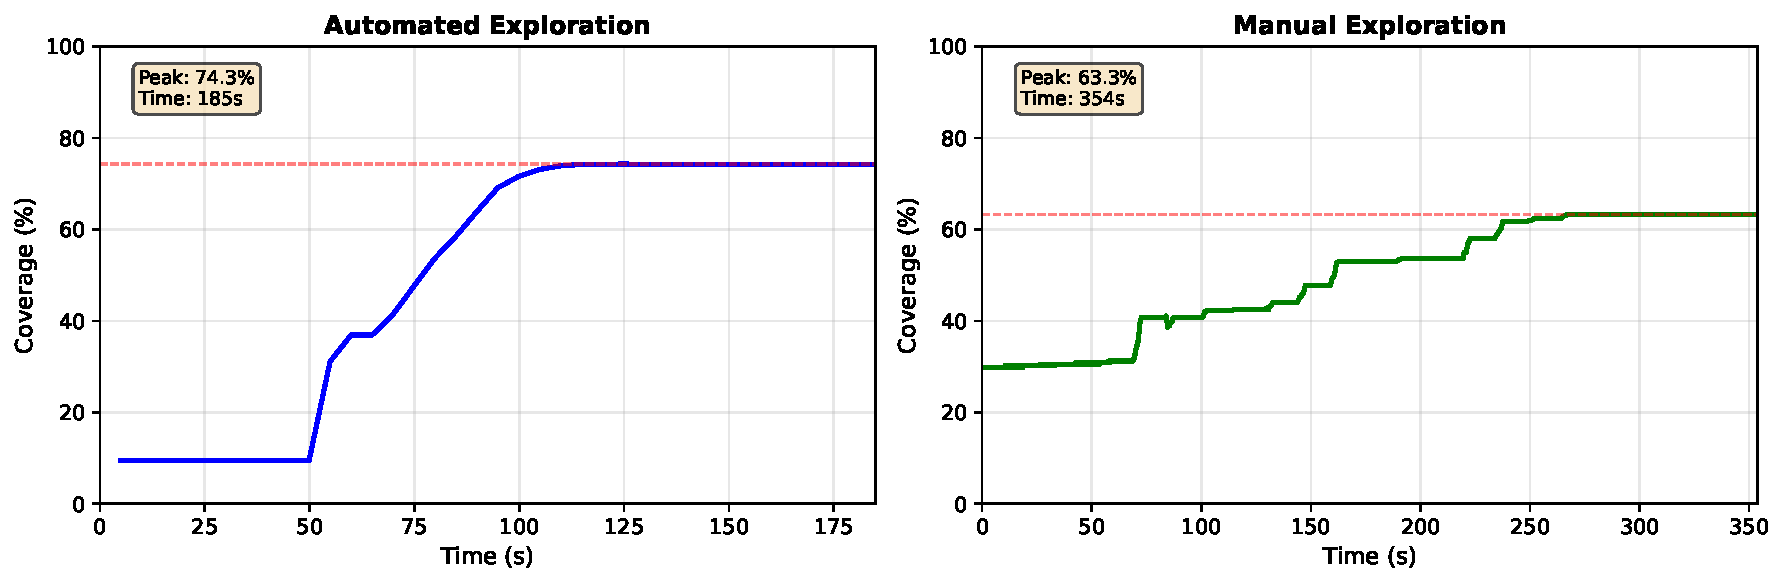
\includegraphics[width=\columnwidth]{figures/coverage_comparison.pdf}
\caption{Coverage over time for automated (left) and manual (right) exploration. Automated exploration achieves higher peak coverage (74.3\%) in less time (185s) compared to manual teleoperation (63.3\%, 354s).}
\label{fig:coverage}
\end{figure}

\subsection{Analysis \& Observations}

\textbf{Initial Delay Issue:} The 50-second startup delay before coverage increases requires investigation. Hypotheses include: (1) SLAM initialization lag, (2) initial frontier detection failures, or (3) Nav2 costmap synchronization delays.

\textbf{Coverage Saturation:} Neither condition achieved full coverage ($>$95\%). Inspection of exploration videos reveals unreachable narrow corridors filtered out by min\_frontier\_size and potential local minima where the robot cannot find viable frontiers.

\textbf{Computational Performance:} Running in a conda ROS2 environment on local hardware (vs. native installation) may contribute to reported "slow" exploration. Profiling is needed to identify bottlenecks in frontier search, costmap processing, or path planning.

\textbf{Parameter Sensitivity:} The current planner\_frequency (0.15 Hz) causes infrequent frontier updates. Increasing this may improve responsiveness but could increase computational load.

\subsection{Limitations}

Our preliminary results are limited to a single environment and parameter configuration. Key limitations include:

\begin{itemize}
    \item \textbf{Single environment:} Results may not generalize to open spaces, cluttered environments, or multi-room structures.
    \item \textbf{Simulation only:} Real-world deployment would introduce sensor noise, localization drift, and mechanical constraints.
    \item \textbf{Limited parameter sweep:} We have not systematically explored the impact of gain\_scale, potential\_scale, or planner\_frequency.
    \item \textbf{No failure analysis:} We have not quantified navigation failures, frontier selection errors, or recovery behaviors.
\end{itemize}

\section{Plan Forward}

\subsection{Milestone 2 Objectives}

\textbf{1. Performance Optimization (Weeks 1-2):}
\begin{itemize}
    \item Profile computational bottlenecks using ROS2 profiling tools
    \item Investigate initial delay and implement warm-start strategies
    \item Conduct parameter sweep: vary planner\_frequency (0.1-1.0 Hz), min\_frontier\_size (0.3-1.5m), and scoring weights
    \item Compare native ROS2 installation vs. conda environment performance
\end{itemize}

\textbf{2. Multi-Environment Evaluation (Weeks 2-3):}
\begin{itemize}
    \item Test in 3-5 environments: open world, maze, multi-room house, warehouse
    \item Measure coverage, time-to-completion, path efficiency (distance traveled / coverage gained)
    \item Analyze failure modes and recovery strategies
\end{itemize}

\textbf{3. Advanced Features (Week 3):}
\begin{itemize}
    \item Implement dynamic parameter adaptation based on exploration phase
    \item Explore alternative frontier selection heuristics (information gain, expected coverage)
    \item Investigate multi-robot exploration using map\_merge component
\end{itemize}

\subsection{Final Report Deliverables}

By the final report, we expect to deliver:
\begin{itemize}
    \item Comprehensive performance characterization across 5+ environments
    \item Optimized parameter configurations with ablation studies
    \item Comparison with alternative exploration strategies (random walk, wall-following)
    \item Real-world deployment feasibility analysis
    \item Open-source code release with documentation
\end{itemize}

\subsection{Risk Mitigation}

\textbf{Risk:} Computational constraints prevent real-time exploration. \textbf{Mitigation:} Optimize frontier search algorithms, reduce planner frequency, or migrate to more powerful hardware.

\textbf{Risk:} Limited environment diversity in simulation. \textbf{Mitigation:} Use existing Gazebo world repositories and procedurally generated environments.

\textbf{Risk:} Time constraints for real-world deployment. \textbf{Mitigation:} Prioritize simulation results; real-world tests are optional stretch goals.

\section{Conclusion}

We have successfully implemented a functional autonomous exploration system in ROS2, achieving automated coverage of 74.3\% with 2.24$\times$ higher efficiency than manual teleoperation. Our custom metrics pipeline enables quantitative performance evaluation, revealing both strengths (systematic coverage) and weaknesses (initial delays, parameter sensitivity). Milestone 2 will focus on optimization, multi-environment generalization, and addressing identified limitations to produce a robust, well-characterized exploration system.

\section*{Acknowledgments}

We thank the m-explore-ros2 open-source community for providing the foundational codebase and the ROS2 ecosystem for robust robotics middleware.

\bibliographystyle{plainnat}
\begin{thebibliography}{1}

\bibitem{horner2016exploration}
Jiri Horner.
\newblock \href{https://github.com/hrnr/m-explore}{m-explore: Multi-robot exploration package for ROS}.
\newblock GitHub repository, 2016.

\bibitem{yamauchi1997frontier}
Brian Yamauchi.
\newblock A frontier-based approach for autonomous exploration.
\newblock In \emph{Proceedings of the 1997 IEEE International Symposium on Computational Intelligence in Robotics and Automation}, pages 146--151. IEEE, 1997.

\bibitem{burgard2005coordinated}
Wolfram Burgard, Mark Moors, Dieter Fox, Reid Simmons, and Sebastian Thrun.
\newblock Collaborative multi-robot exploration.
\newblock In \emph{Proceedings of the 2000 IEEE International Conference on Robotics and Automation}, volume~1, pages 476--481. IEEE, 2000.

\end{thebibliography}

\end{document}
